%
% copied from: https://tikz.net/spherical_volume/
% date: 2023, June 26
%
% adjusted by Alexander Smolka
%
\documentclass[crop,tikz]{standalone}
\usepackage{tikz}
	\usetikzlibrary{shapes}
	\usetikzlibrary{automata}
	\usetikzlibrary{arrows}
	\usetikzlibrary{backgrounds}
	\usetikzlibrary{calc}
	\usetikzlibrary{positioning}
	\usetikzlibrary{patterns}
	\usetikzlibrary{decorations.pathmorphing}
	\usetikzlibrary{decorations.pathreplacing}

\usepackage{siunitx}


\input{../../../../../resources/latex/_symbols.qmd}

\begin{document}

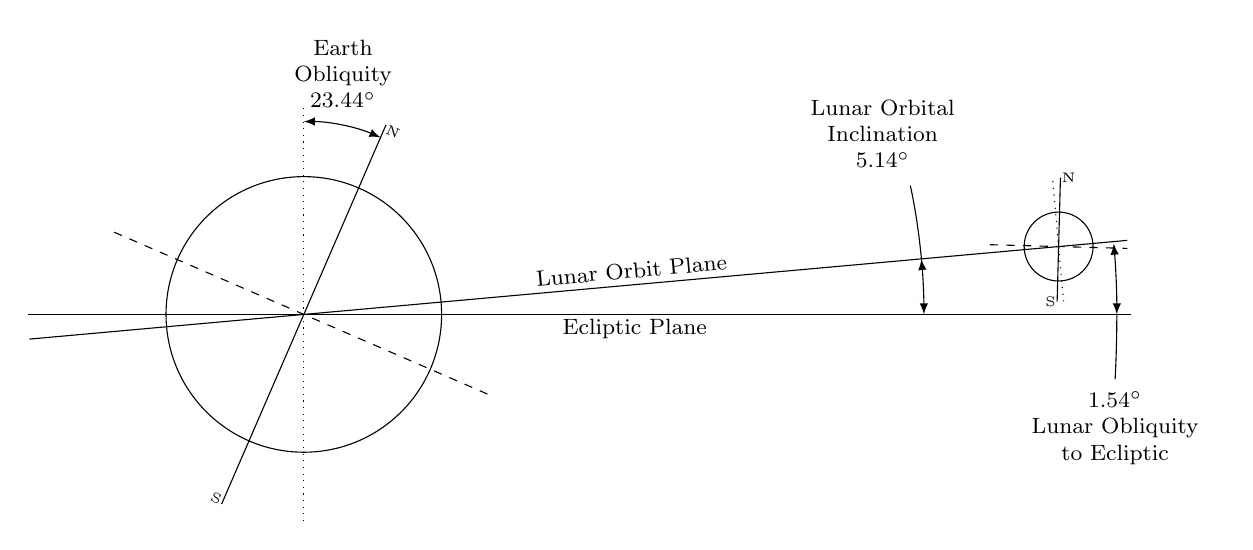
\begin{tikzpicture}[
    scale=1.75]

    % ecliptic plane
    \draw (0,0) -- (8,0) 
        node[midway, below, xshift=20pt, yshift=2pt] {\footnotesize Ecliptic Plane};

    % earth
    \draw (2,0) circle (1);
    \draw[dotted] (2,-1.5) -- (2,1.5);
    \draw[rotate around={-23.44:(2,0)}] (2,-1.5) -- (2,1.5)
        node[at end, right, xshift=-3pt, rotate=-23.44]{\tiny{N}}
        node[at start, left, xshift=3pt, rotate=-23.44]{\tiny{S}};
    \draw[rotate around={-113.44:(2,0)}, dashed] (2,-1.5) -- (2,1.5);

    % moon
    \begin{scope}[rotate around={5.14:(2,0)}]
        % lunar orbit plane
        \draw (0,0) -- (8,0) 
            node[midway, above, rotate around={5.14:(2,0)}, xshift=20pt, yshift=4pt] {\footnotesize Lunar Orbit Plane};
        
        %
        \draw (7.5,0) circle (0.25);
        \draw[dotted] (7.5,-0.4) -- (7.5,0.5);
        \draw[rotate around={-6.68:(7.5,0)}] 
            (7.5,-0.4) -- (7.5,0.5)
            node[at end, right, xshift=-3pt]{\tiny{N}}
            node[at start, left, xshift=3pt]{\tiny{S}};
        \draw[rotate around={-96.68:(7.5,0)}, dashed] (7.5,-0.5) -- (7.5,0.5);
    \end{scope}

    % angles / arcs
    \draw[latex-latex] (2,0) ++(90:1.4) arc (90:66.56:1.4) 
        node[midway, above] {\footnotesize \begin{tabular}{c} Earth \\  Obliquity \\ \SI{23.44}{\degree} \end{tabular}};

    \draw[latex-latex] (2,0) ++(0:4.5) arc (0:5.14:4.5);
    \draw[thin] (2,0) ++(5.14:4.5) arc (5.14:12:4.5) 
        node[at end, above, xshift=-10pt] {\footnotesize \begin{tabular}{c}Lunar Orbital \\ Inclination \\ \SI{5.14}{\degree}\end{tabular}};

    \draw[latex-latex] (2,0) ++(5:5.9) arc (5:0:5.9);
    \draw[thin] (2,0) ++(0:5.9) arc (0:-3:9) 
        node[at end, below] {\footnotesize \begin{tabular}{c}\SI{1.54}{\degree} \\ Lunar Obliquity \\ to Ecliptic \end{tabular}};

\end{tikzpicture}

\end{document}